\documentclass[a4paper,12pt]{article}

\usepackage[czech]{babel}
\usepackage[utf8]{inputenc}

\usepackage{graphicx}	%kvůli pdf souboru z MATLABu
\usepackage{amsmath}	%matice
\usepackage{setspace}	%rozteče v maticích
\usepackage{float}		%obrázky
\usepackage{verbatim}   %víceřádkové komentáře
\usepackage{siunitx}	%hezký jednotky

\sisetup{locale = DE}

\title{Simulační úloha - Servo Amira}
\author{Matouš Vrba}
\date{\today}

% === Formát stránky ===
\usepackage[a4paper]{geometry}
\geometry{
	verbose,
	tmargin=2.2cm,
	bmargin=1.5cm,
	lmargin=1.5cm,
	rmargin=1.5cm}

\begin{document}

\maketitle
\pagebreak
\section{Linearizace modelu}
Stabilní rovnovážná poloha kyvadla je v pracovním bodě $\mathbf{x_0} = [x_{1p}, x_{2p}, x_{3p}, x_{4p}] = [0, -\frac{\pi}{2}, 0, 0]$, ${u_0} = 0$.
\newline
Matice linearizovaného systému v pracovním bodě $\mathbf{x_0}, u_0$:

\renewcommand{\arraystretch}{1.3}
{\Large
\begin{align*}
&A = 
\begin{pmatrix}
\frac{\partial x_1}{\partial x_1} & \frac{\partial x_1}{\partial x_2} & \frac{\partial x_1}{\partial x_3} & \frac{\partial x_1}{\partial x_4}	\\
\frac{\partial x_2}{\partial x_1} & \frac{\partial x_2}{\partial x_2} & \frac{\partial x_2}{\partial x_3} & \frac{\partial x_2}{\partial x_4}	\\
\frac{\partial x_3}{\partial x_1} & \frac{\partial x_3}{\partial x_2} & \frac{\partial x_3}{\partial x_3} & \frac{\partial x_3}{\partial x_4}	\\
\frac{\partial x_4}{\partial x_1} & \frac{\partial x_4}{\partial x_2} & \frac{\partial x_4}{\partial x_3} & \frac{\partial x_4}{\partial x_4}
\end{pmatrix}_{\biggr\rvert_\mathbf{x_0}} =
\left(\begin{array}{cccc} 0 & 0 & 1 & 0\\ 0 & 0 & 0 & 1\\ 0 & \frac{\mathrm{k_2}\, \mathrm{k_3}}{\mathrm{J_p}\, \mathrm{k_1} - {\mathrm{k_2}}^2} & -\frac{\mathrm{J_p}\, b}{\mathrm{J_p}\, \mathrm{k_1} - {\mathrm{k_2}}^2} & \frac{2\, \mathrm{\delta}\, \mathrm{k_2}}{\mathrm{J_p}\, \mathrm{k_1} - {\mathrm{k_2}}^2}\\ 0 & -\frac{\mathrm{k_3}}{\mathrm{J_p} - \frac{{\mathrm{k_2}}^2}{\mathrm{k_1}}} & \frac{b\, \mathrm{k_2}}{\mathrm{k_1}\, \left(\mathrm{J_p} - \frac{{\mathrm{k_2}}^2}{\mathrm{k_1}}\right)} & -\frac{2\, \mathrm{\delta}}{\mathrm{J_p} - \frac{{\mathrm{k_2}}^2}{\mathrm{k_1}}} \end{array}\right)	\\ \\
&B =
\begin{pmatrix}
\frac{\partial x_1}{\partial u}	\\
\frac{\partial x_2}{\partial u}	\\
\frac{\partial x_3}{\partial u}	\\
\frac{\partial x_4}{\partial u}
\end{pmatrix}_{\biggr\rvert_{u_0}} =
\left(\begin{array}{c} 0\\ 0\\ \frac{\mathrm{J_p}}{\mathrm{J_p}\, \mathrm{k_1} - {\mathrm{k_2}}^2}\\ -\frac{\mathrm{k_2}}{\mathrm{k_1}\, \left(\mathrm{J_p} - \frac{{\mathrm{k_2}}^2}{\mathrm{k_1}}\right)} \end{array}\right)	\\ \\
&C =
\begin{pmatrix}
\frac{\partial y_1}{\partial x_1} & \frac{\partial y_1}{\partial x_2} & \frac{\partial y_1}{\partial x_3} & \frac{\partial y_1}{\partial x_4}	\\
\frac{\partial y_2}{\partial x_1} & \frac{\partial y_2}{\partial x_2} & \frac{\partial y_2}{\partial x_3} & \frac{\partial y_2}{\partial x_4}
\end{pmatrix}_{\biggr\rvert_\mathbf{x_0}} =
\left(\begin{array}{cccc} 1 & 0 & 0 & 0\\ 0 & 1 & 0 & 0 \end{array}\right)	\\ \\
&D =
\begin{pmatrix}
\frac{\partial y_1}{\partial u}	\\
\frac{\partial y_2}{\partial u}
\end{pmatrix}_{\biggr\rvert_{u_0}} =
\left(\begin{array}{c} 0\\ 0 \end{array}\right)
\end{align*}
}

\newpage
\section{Saturace, pásma necitlivosti, apod.}
Vstup systému v MATLABu je normalizován na interval $u_{norm} \in \left<-1; 1\right>$, což vymezuje saturaci vstupu. Pásmo necitlivosti jsme identifikovali v intervalu $\left<-0.007; 0.007\right>$.
\newline
\newline
Při výchylce kyvadla v rozmezí $\pm \SI{12}{\degree}$ je vliv kyvadla na polohu kyvadla zanedbatelný a dá se považovat za pásmo necitlivosti. Toho jsme využili také při identifikaci dynamiky kyvadla z počátečních podmínek.
\newline
\newline
Další nelinearitu jsme identifikovali u ramene, které se na jednu stranu posouvalo snáze, než na druhou.

\section{Identifikace dynamiky motoru (ramene)}
Uvažujeme první rovnici, popisující systém před úpravou do stavových rovnic, v okolí pracovního bodu $\mathbf{x_0}$. Po zanedbání křížových členů (vliv kyvadla na polohu ramene je pro identifikaci ostatních členů zanedbatelný) a linearizaci goniometrických funkcí získáváme následující předpis:
\begin{align*}
(J_m + mr^2)\ddot{\varphi}_m(t) + b\dot{\varphi}_m(t) = M(t) = k_u\cdot u_{norm}(t)
\end{align*}
Po zlaplaceování a standardních úpravách dostaneme přenos a srovnání s normálním tvarem:
\begin{align*}
H_{\varphi_m}(s) = \frac{k_u}{b}\cdot \frac{1}{s(\frac{J_m + mr^2}{b}s + 1)} = k\frac{1}{s(Ts + 1)}
\end{align*}
Jedná se tedy o systém druhého řádu s jedním pólem v nule. Takový systém se dá snadno identifikovat ze skokové odezvy. Srovnáním identifikovaných obecných konstant $T$ a $k$ s odpovídajícími konstantami v našem systému je pak můžeme vypočítat:
\begin{align*}
&b = \frac{k_u}{k} = k_u\frac{T}{\tau} = \SI{0,5024}{\kilo \gram \meter \squared \per \second}	\\
&k_1 = (J_m + mr^2) = T\cdot b = 0,0831
\end{align*}
, kde $T$ a $\tau$ odečteme z grafu (viz. obrázek níže).
\begin{figure}[H]
	\centering
    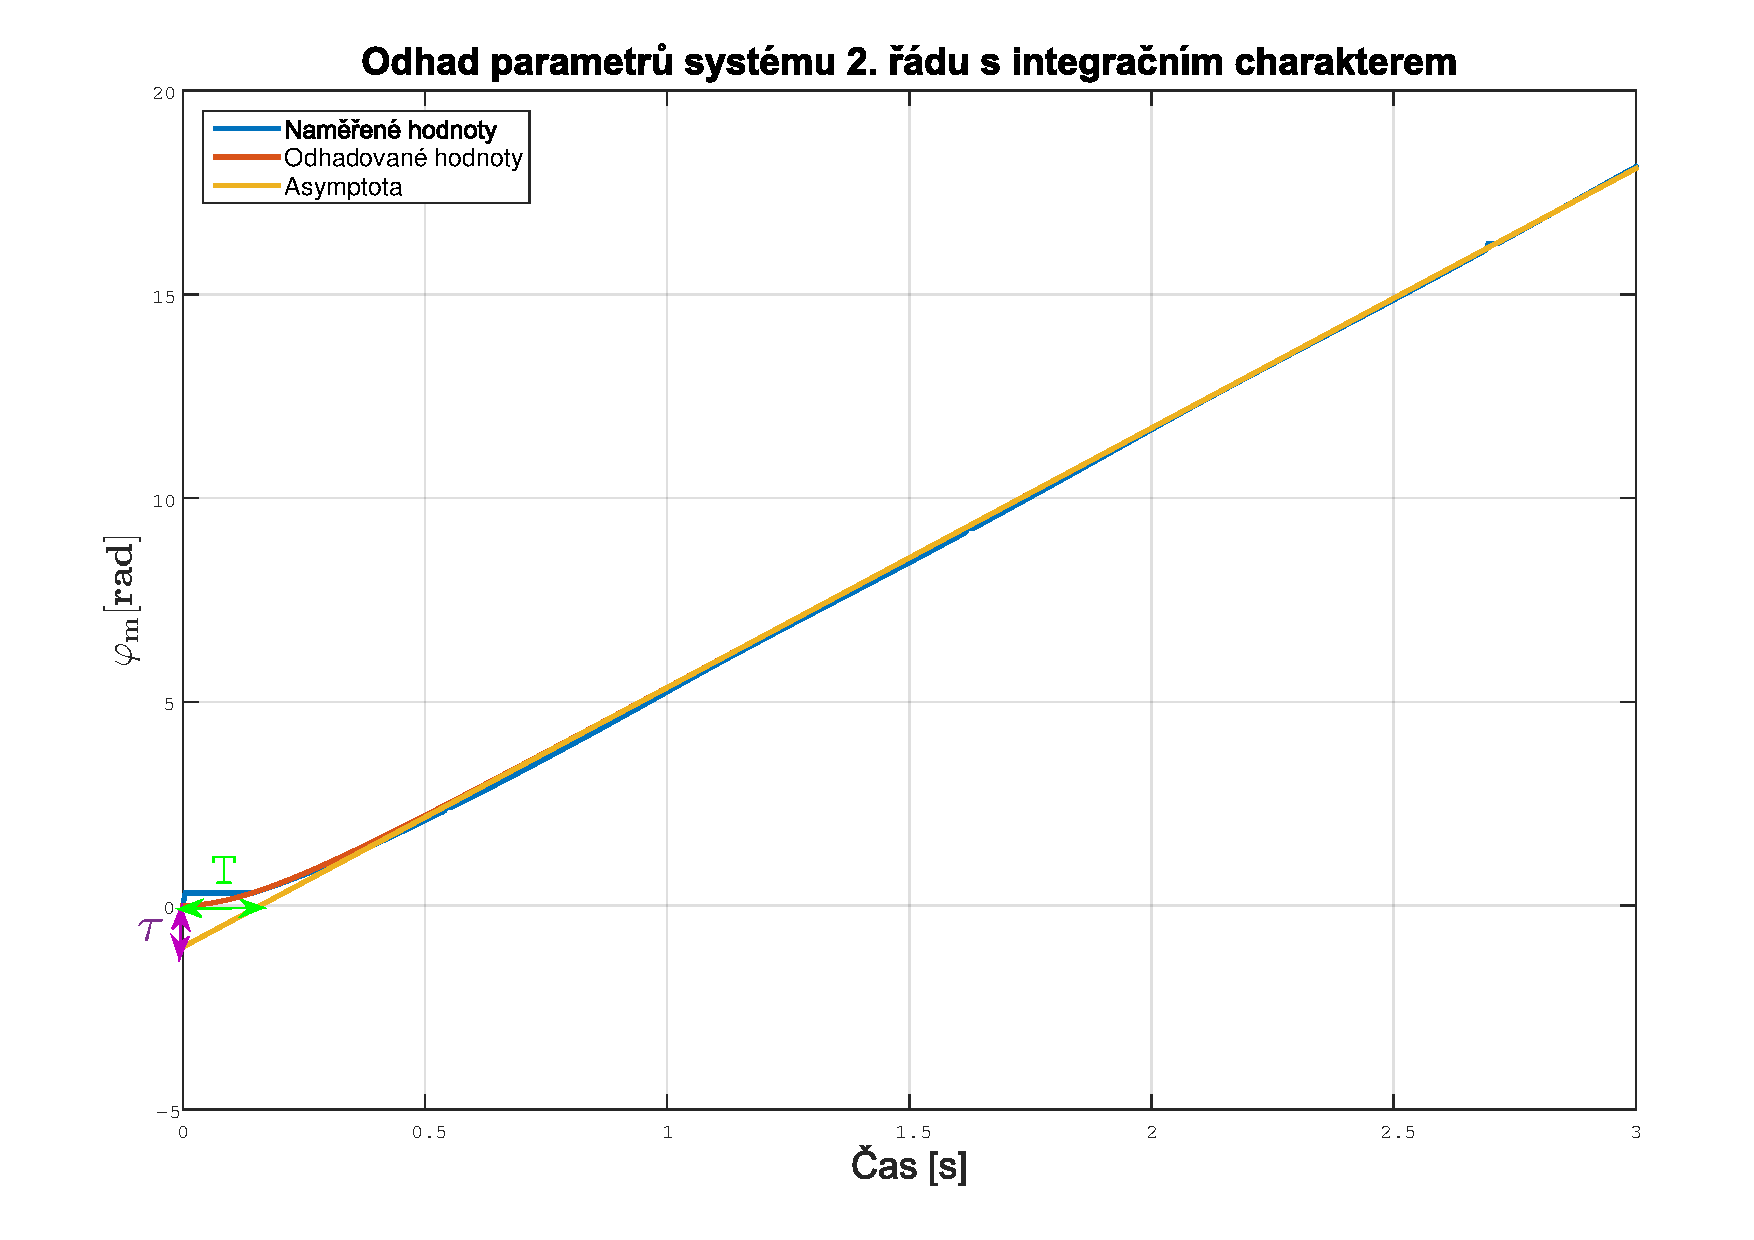
\includegraphics[scale=.4]{Odhad_phim}
    \caption{Odhad parametrů rovnice pro $\varphi_m$ z asymptoty}
\end{figure}

\section{Identifikace křížových členů}
Zbývá nám ještě určit konstanty $k_2$ a $k_3$, které v rovnicích tvoří koeficienty křížových členů. Platí, že
\begin{align*}
&k_2 = mlr && k_3 = mgl
\end{align*}
Prvky $l$ a $r$ jsme určili naměřením na modelu kyvadla (jedná se o délku kyvadla a délku ramene), $g$ je tíhové zrychlení, které je pro naši polohu známé, a nakonec hodnotu $m$ jsme dostali zadanou. Výsledné hodnoty tedy jsou:
\begin{align*}
&m = \SI{0,175}{ \kilo \gram} &&g = \SI{9,81}{\meter \per \second}	\\
&l = \SI{0,17}{\meter} &&r = \SI{0,2}{\meter}
\end{align*}
\begin{figure}[H]
	\centering
    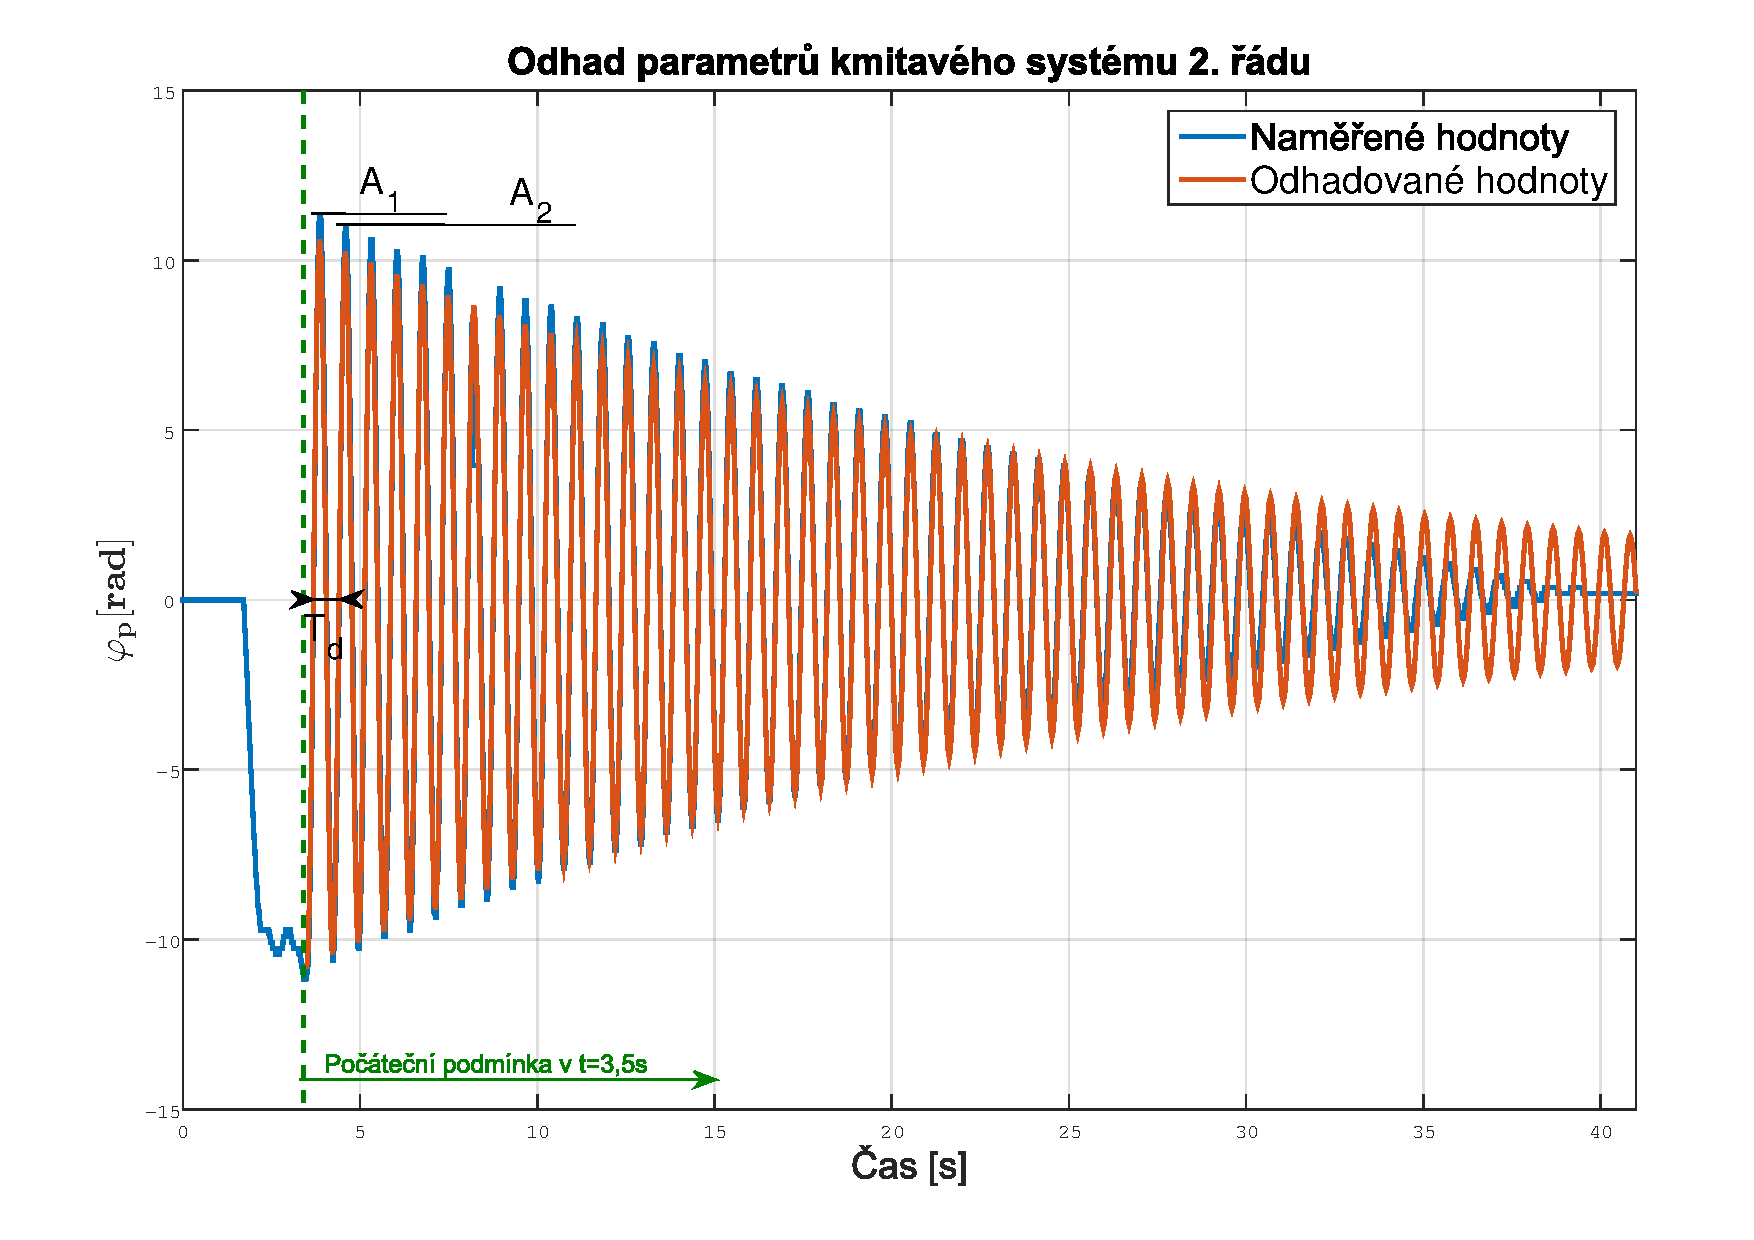
\includegraphics[scale=.6]{Odhad_phip}
    \caption{Odhad parametrů rovnice pro $\varphi_m$ z asymptoty}
\end{figure}





Určené hodnoty jsme ještě upravili tak, aby dobře seděly i pro obecnější případ bez zanedbaných a linerizovaných členů. Tyto upravené hodnoty jsou:
\begin{align*}
&b = \SI{0,5193}{\kilo \gram \meter \squared \per \second} \\
&J_p = \SI{0,0044}{\kilo \gram \metre \per \second \squared}	&&	\delta = \SI{1,9297e-4}{\kg \m \squared \per \second}
\end{align*}





\section{Závěr}
I přesto, že jsme se snažili parametry systému určit co nejpřesněji, neodpovídají naše modely naměřeným hodnotám reálného systému pro větší vstupy příliš dobře, jak je vidět z porovnávání odezev na skok v sekci 8 (hlavně v poloze kyvadla $\varphi_p$). To může být způsobeno dalšími skrytými nelinearitami systému, použitím rovnic pro kyvadlo na vozíku, které nemusí dostatečně přesně popisovat rotační kyvadlo, zanedbáním případné dynamiky vstupu a zanedbáním vlivu tření vzduchu, které nejspíš způsobuje ustálení polohy kyvadla v jiné poloze, než je klidová, když je rychlost ramene nenulová.
\newline
Pro malé vstupy, a ze začátku i pro větší, se ale odezvy systémů celkem shodují, takže snad bude tyto modely možné použít pro řízení v dalších částech laboratorní úlohy.



\end{document}